\documentclass{article}

\usepackage[usenames]{color} 
\usepackage{graphicx} 
\usepackage{pdfpages} 

\newcommand{\todo}[1]{\textcolor{red}{\textbf{TODO: }\it{#1}}}
\newcommand{\inhoud}[1]{\textcolor{blue}{\textbf{Summary: }\it{#1}}}
\newcommand{\revise}[1]{\textcolor{orange}{\textbf{Revise: }\it{#1}}}

\definecolor{MyDarkGreen}{rgb}{0.13, 0.54,0.13} 
\newcommand{\voegtoe}[1]{\textcolor{MyDarkGreen}{\textbf{-Insert: }\it{#1}}\newline}

\title{Design decisions Dynamic Cell Structures \small{Properties and Interaction}}
\author{Ruud op den Kelder}

\begin{document}
\maketitle

For the 2D spatial growth model based editor I have chosen to represent the growth models with cell structures. 

The behavior of the cell structures is governed by these four things:  

\begin{enumerate}
\item Mass Spring System. A mass spring system which connects neighbouring cells belonging to the same system. It has the responsibility of keeping the topology of the group of cells intact.  
\item Properties and behaviour of the cells and cellsystems; shape, size, events (events occur when two or more cell structures collide.) 
\item User input. What ever the editor tool provides to the user to manipulate the cellstructures.
\item Automatic map generation. AI techniques to govern the map generation process.  
\end{enumerate}  

\section{Properties of Cell Structures}

\subsection{Properties of a Cell}
 
An important part of the cell structure concept is the viral nature of the cells. This means that a cell i can transfer properties to neighbouring cell j thereby altering the behaviour of cell j. In this section I will first discuss the physical properties of the cells (shape, mass, size and friction). These properties affect the way cells translate and rotate in our 2D space, thereby shaping the boundary of the cell systems. Then I will discuss the different types of other viral properties of cells.    


\subsubsection{Physical Properties}
A cell can have any of the shapes in figure 1.

\begin{figure}[h,t]
\centering
  \begin{center}

	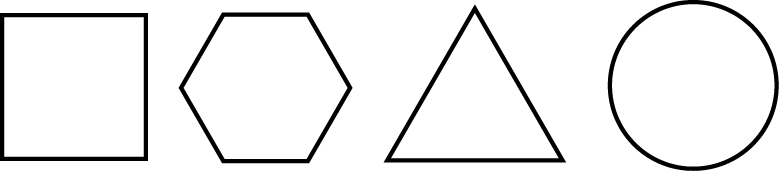
\includegraphics[width=250pt]{images/shapes.png}
\end{center}
	\caption{basic shapes for the cells}
\end{figure}


The combination of shape, size and mass of a cell is important because it determines the way cells physically react to collisions.

\subsubsection{Viral Properties}

Viral properties are properties which can be transferred from one cell system to another. Examples of viral properties could be shape of the cells, speed of growth or friction on the cells. 

\subsection{Properties of a System}

The behaviour of a Cell system is defined by its property set. 
It is the goal of this research to find certain configurations of properties which represent growth of natural phenomenon in an intuitive way. Such that the property set of a system could be labeled by names such as: land, water, vegetation, desert, mountains. Land could be a cellsystem that provides a surface desert and mountains to grow on. I will experiment with different configurations of parameters for the growing of natural phenomena. I will look at different kind of shapes and sizes for the cells of a system to see how they affect the growth process and the interaction between systems (both physically and virally). 

For example, I could use large hexagon shaped cells to represent land and small triangle shaped cells to represent water. The land-system shall have a low density which means that there is much space between the cells which can be accomplished by making the springs that hold the cells relatively long. This way, water cells can enter the land-system which can then result in an event such as spawning a new type of cell system (river, vegetation, etc..). Also the collision between a water cell and a land cell can cause the expansion of the land to halt locally. With my experiments I hope to find out whether configurations such as this will lead to meaningful results. Ofcourse you can also think of more abstract property sets which do not nessecerily represent any natural phenomenon, but my primary goal is to find configurations of cellsystems that are useful for the generation of 2D outdoor maps.  

I will now address the core behaviour of a cell structure. The core behaviour is the expansion of the cellsystem over time. Cellsystems consist of a set of cells connected with springs. The expansion is regulated by properties such as growth rate, maximal volume, cell spawning, cell sizing etc..    

\subsection{Events}

\begin{itemize}
\item spawning of a cellsystem
\item transfer of properties
\item completion of a cell system
\item destruction of a cell system
\item merging of two cell systems
\end{itemize}


\subsection{Scripting for properties and events}

The cellsystems have many different parameters which control there behaviour. Alteration of these parameters has to be an easy and swift process. Therefore, we will be using a scripting language to handle properties and part of the behaviour of cells. We have chosen Lua for our scripting system, due to its succesful history in game development and straightforward usage.

List of functionalities handled by LUA: 

\begin{itemize}
\item definitions of cells  
\item definitions of the cell systems
\item definitions of events
\item map generation AI implementation
\item Initial configuration of the entire system 
\item Load and Save functionality of the editor   
\end{itemize}

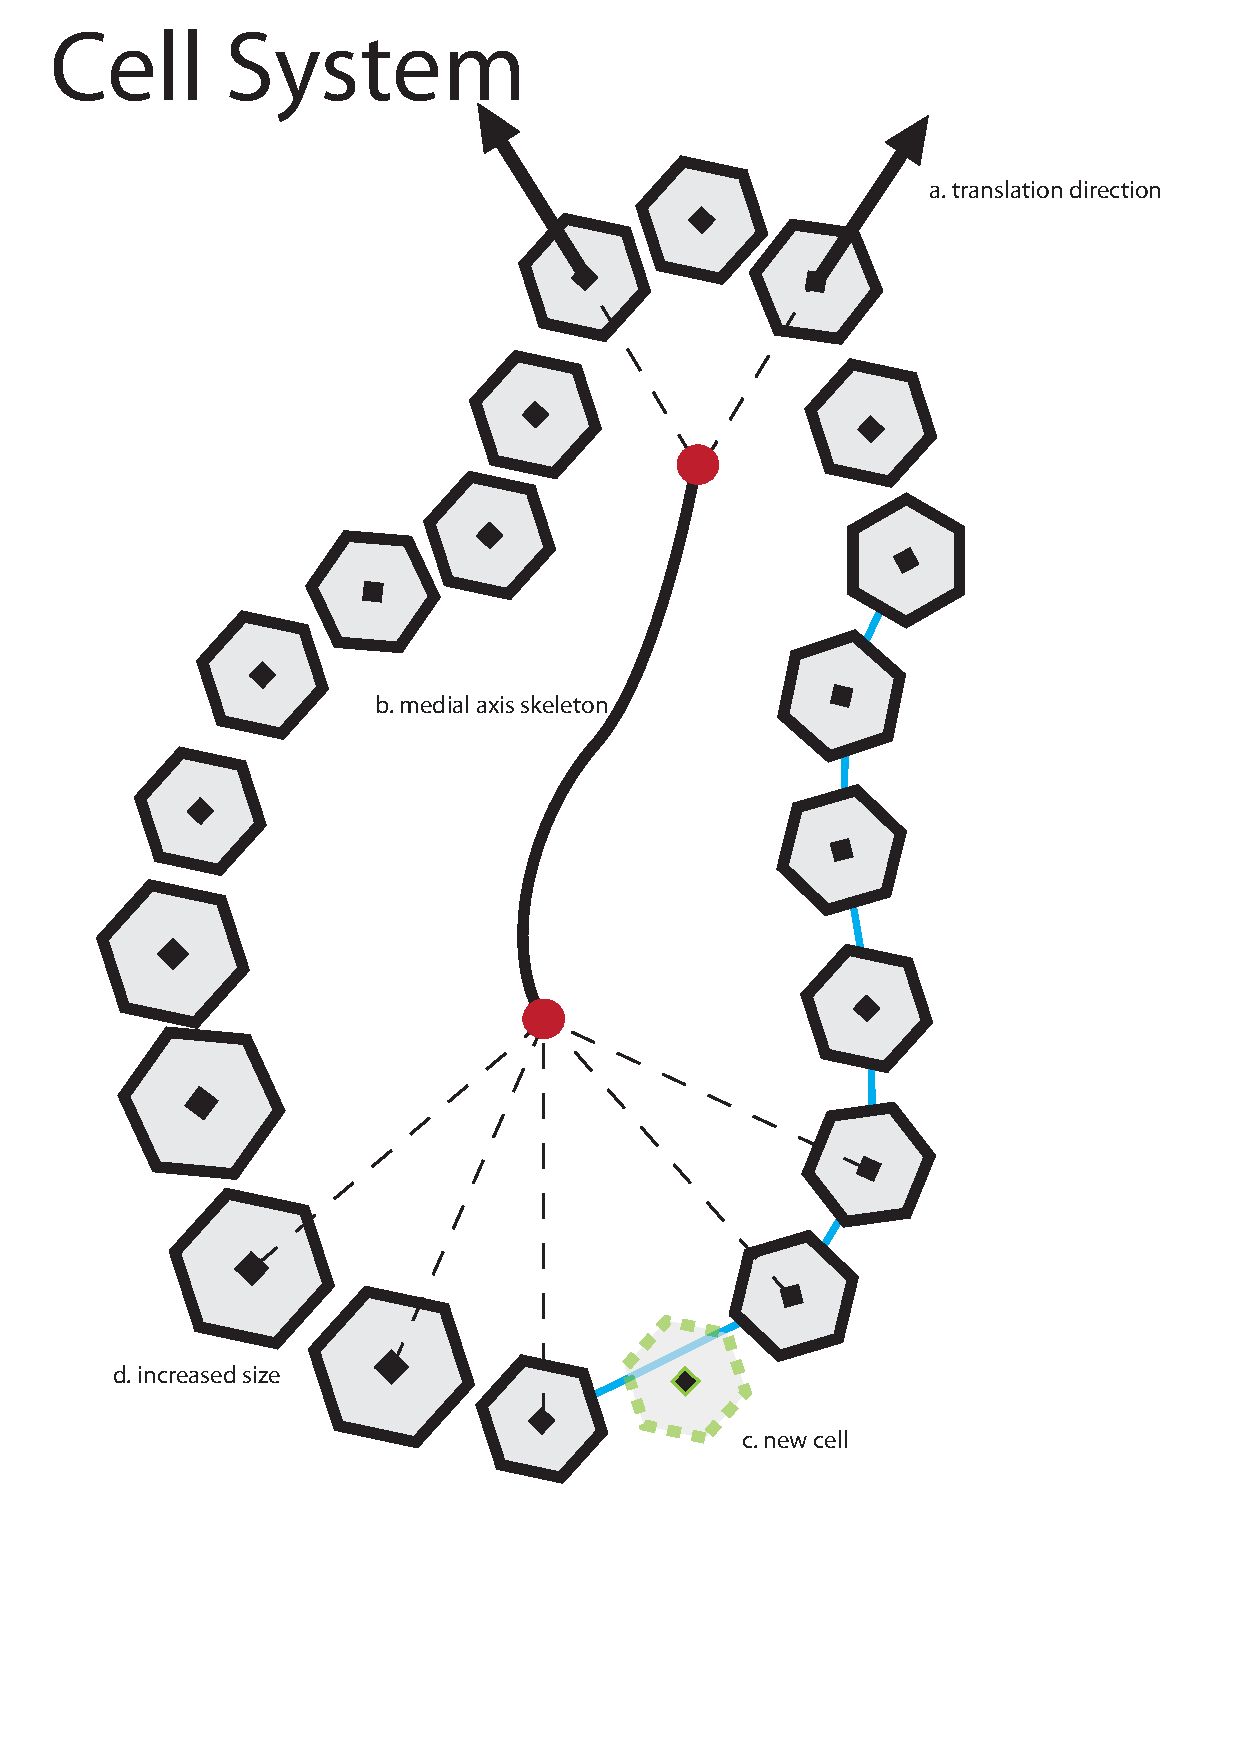
\includepdf[pages=-]{images/cellsystem.pdf}
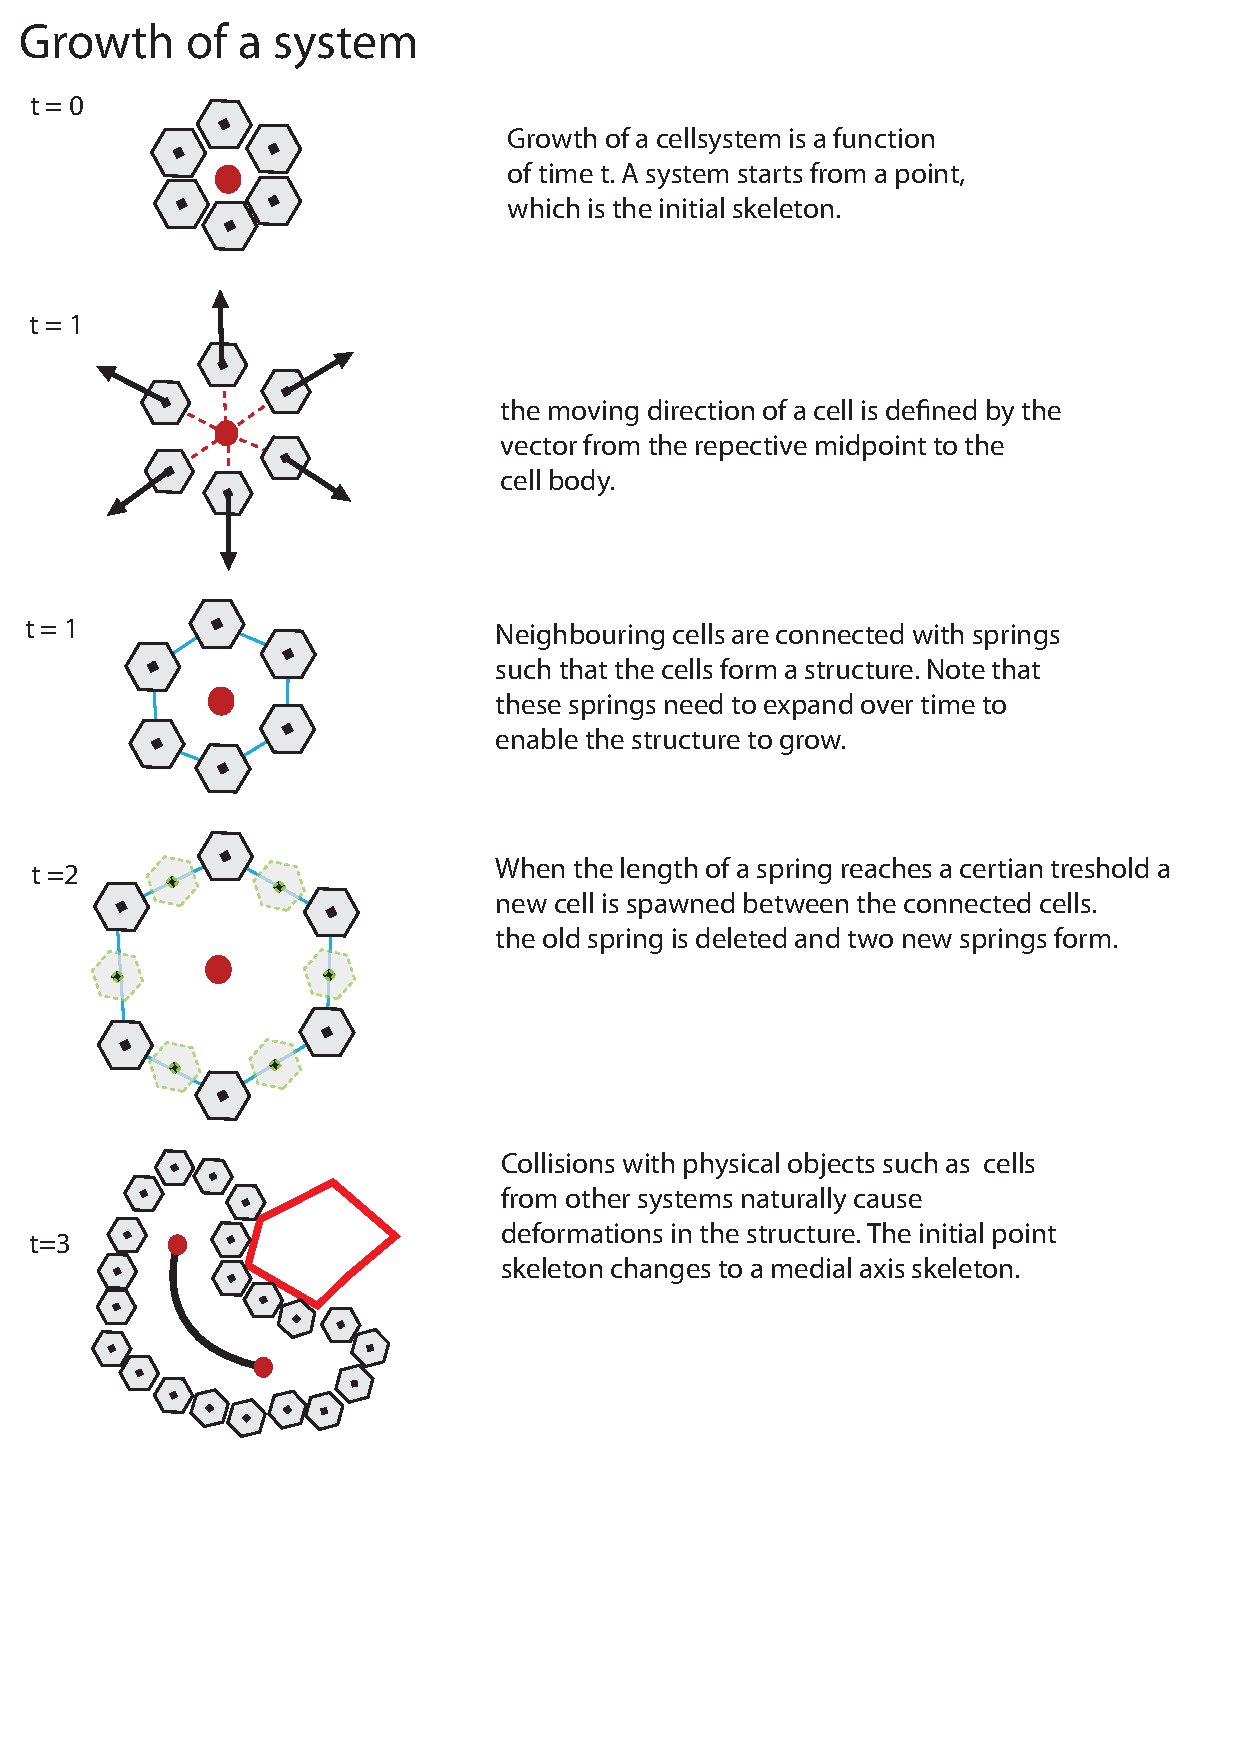
\includepdf[pages=-]{images/growth.pdf}
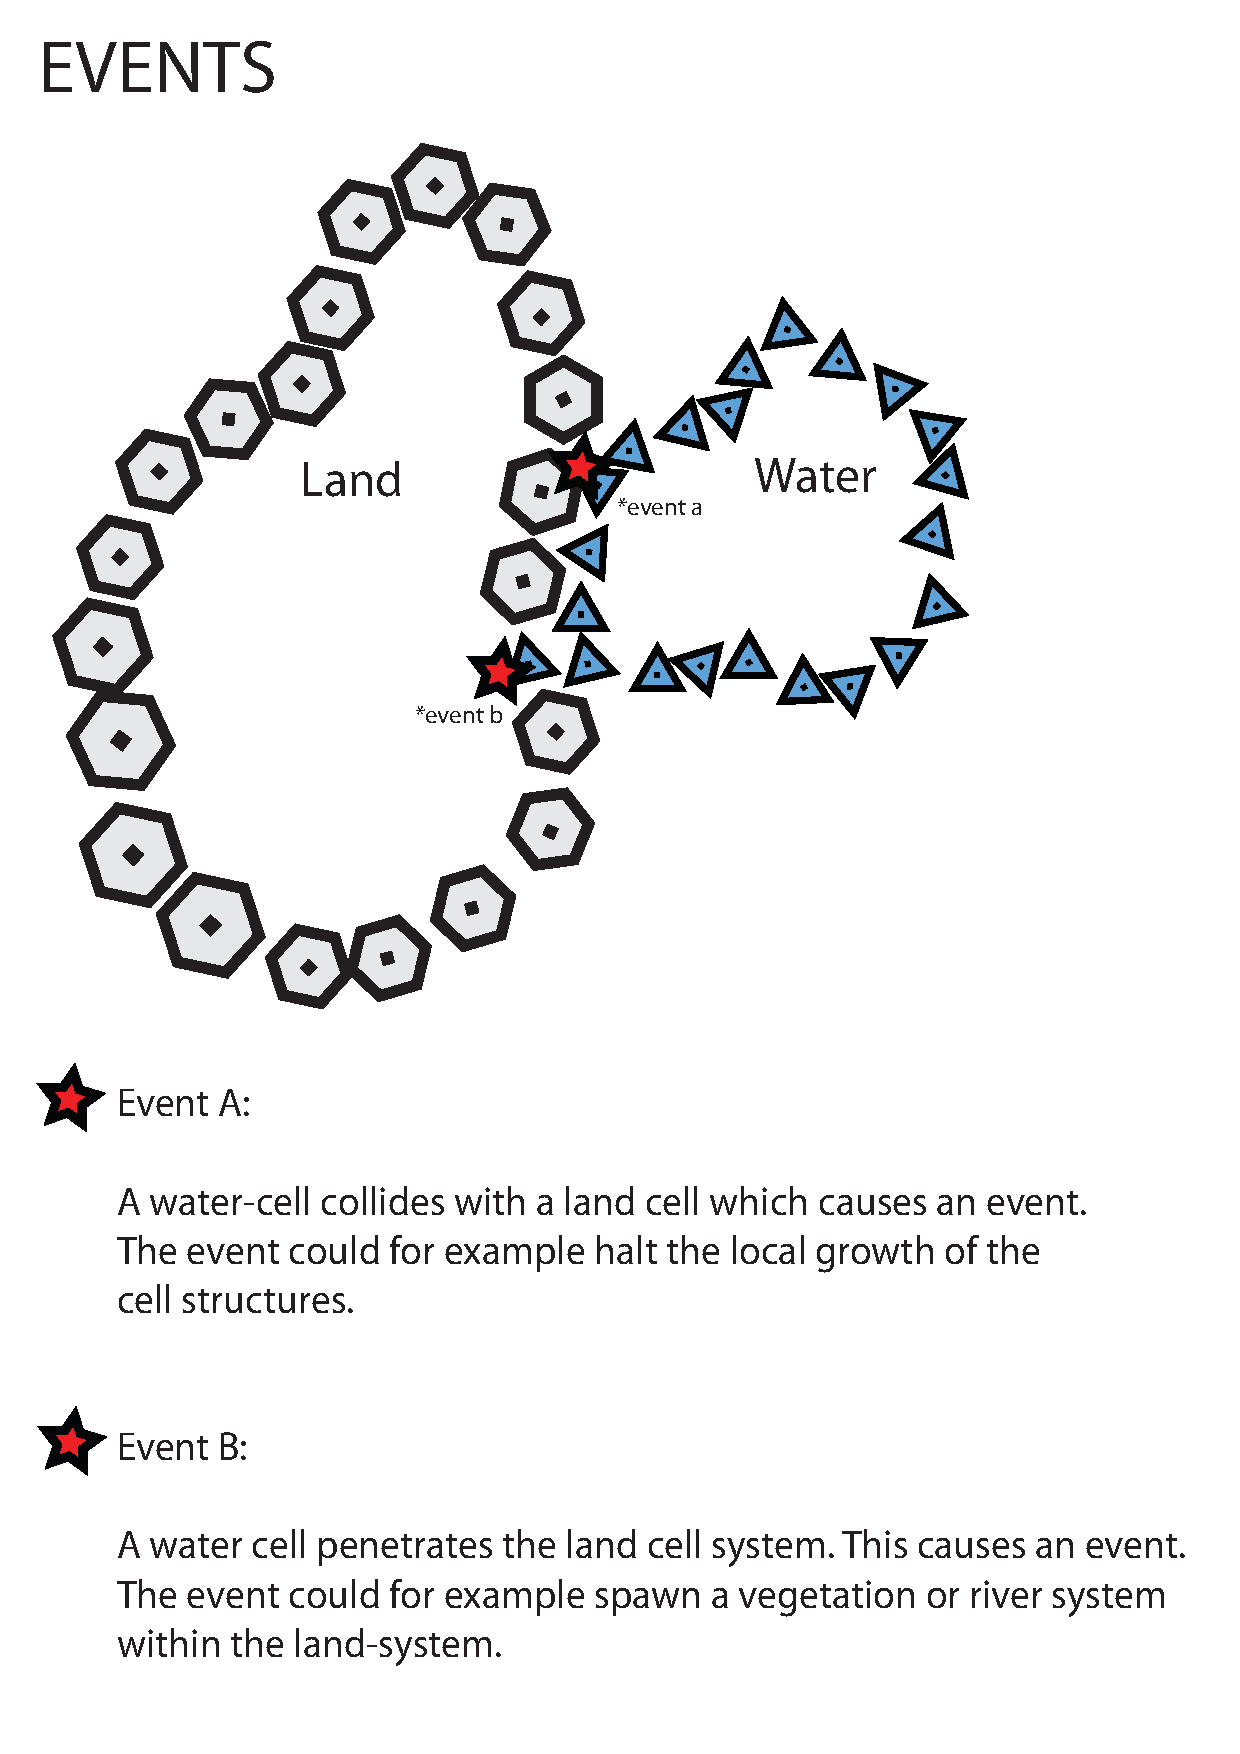
\includepdf[pages=-]{images/events.pdf}

\end{document}
